\part{QR factorization and Least Squares}
\chapter{Projectors}
We now enter the second part of the book, whose theme is orthogonality. We begin with the fundamental tool of projection matrices, or projectors, both orthogonal and nonorthogonal.
\section{Projectors}

%────────────────────────────────────────
\begin{definition}
[Projectors]
\label{def: Projectors}
A projector is a square matrix $P$ that satisfies
\begin{align*}
P^2=P .
\end{align*}
\end{definition}
%────────────────────────────────────────
This definition includes both orthogonal projectors, to be discussed in a moment, and nonorthogonal ones. To avoid confusion one may use the term oblique projector in the nonorthogonal case. 

%────────────────────────────────────────
\begin{figure}[H]
    \centering
    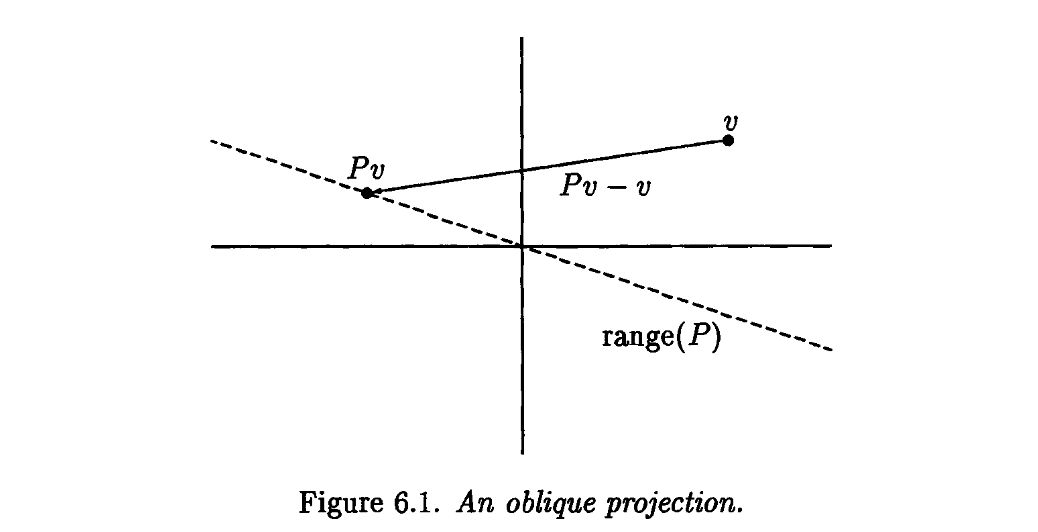
\includegraphics[width=0.8\textwidth]{figures/6-1.png}
\end{figure}
%────────────────────────────────────────

\section{Complementary Projectors} 

%────────────────────────────────────────
\begin{definition}
[Complementary Projectors]
\label{def: Complementary Projectors}
If $P$ is a projector, $I-P$ is also a projector, for it is also idempotent:
\begin{align*}
(I-P)^2=I-2 P+P^2=I-P .
\end{align*}
\end{definition}
%────────────────────────────────────────

We have the following corollary:

%────────────────────────────────────────
\begin{corollary}
\label{cor: P and I-P}
We have the following results: 
\begin{itemize}
    \item $\range(I-P) = \nul (P)$, 
    \item $\nul (I-P) = \range(P)$, 
    \item $\range(P) \cap \nul(P) = \{0\} . $
\end{itemize}
\end{corollary}
%────────────────────────────────────────
These computations show that a projector separates $\mathbb{C}^m$ into two spaces. Conversely, let $S_1$ and $S_2$ be two subspaces of $\mathbb{C}^m$ such that $S_1 \cap S_2=\{0\}$ and $S_1+S_2=\mathbb{C}^m$, where $S_1+S_2$ denotes the span of $S_1$ and $S_2$, that is, the set of vectors $s_1+s_2$ with $s_1 \in S_1$ and $s_2 \in S_2$. (Such a pair are said to be complementary subspaces.) Then there is a projector $P$ such that $\operatorname{range}(P)=$ $S_1$ and $\operatorname{null}(P)=S_2$. We say that $P$ is the projector onto $S_1$ along $S_2$.

\section{Orthogonal Projectors}
An orthogonal projector is one that projects onto a subspace $S_1$ along a space $S_2$, where $S_1$ and $S_2$ are orthogonal. (Warning: orthogonal projectors are not orthogonal matrices!)

%────────────────────────────────────────
\begin{figure}[H]
    \centering
    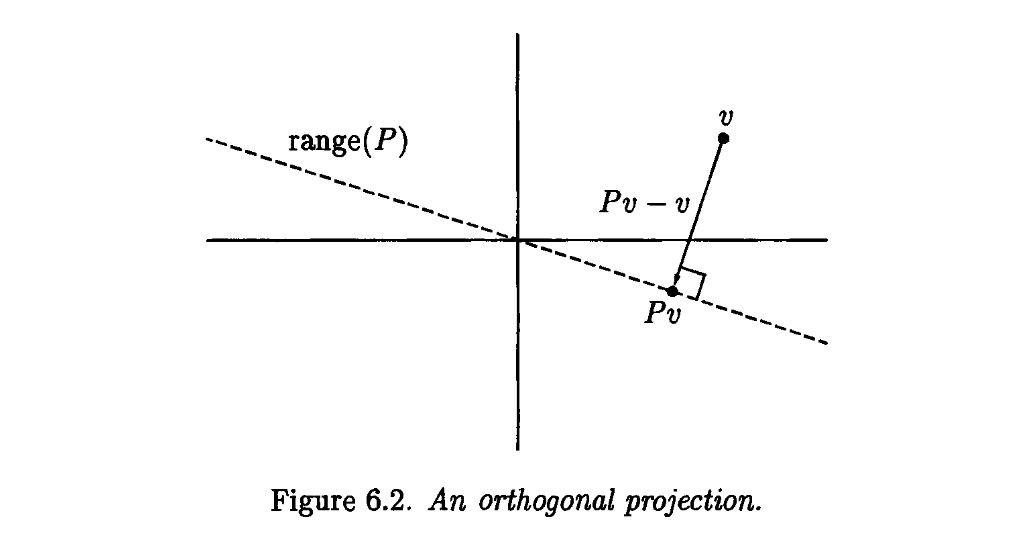
\includegraphics[width=0.8\textwidth]{figures/6-2.png}
\end{figure}
%────────────────────────────────────────


%────────────────────────────────────────
\begin{theorem}
\label{thm: orthogonal projector}
A projector $P$ is orthogonal if and only if $P=P^*$. 
\end{theorem}
%────────────────────────────────────────

\section{Projection with an Orthonormal Basis}
 Let $\left\{q_1, \ldots, q_n\right\}$ be any set of $n$ orthonormal vectors in $\mathbb{C}^m$, and let $\hat{Q}$ be the corresponding $m \times n$ matrix. Thus the map
 \begin{align}
    \label{eq: project with orthonormal basis}
 v \mapsto \sum_{i=1}^n\left(q_i q_i^*\right) v
 \end{align}
 is an orthogonal projector onto range $(\hat{Q})$, and in matrix form, it may be written $y=\hat{Q} \hat{Q}^* v$. 

 An important special case of orthogonal projectors is the rank-one orthogonal projector that isolates the component in a single direction $q$, which can be written
\begin{align*}
P_q=q q^* .
\end{align*}
These are the pieces from which higher-rank projectors can be made, as in (6.7). Their complements are the rank $m-1$ orthogonal projectors that eliminate the component in the direction of $q$ :
\begin{align*}
P_{\perp q}=I-q q^* .
\end{align*}
Equations (6.8) and (6.9) assume that $q$ is a unit vector. For arbitrary nonzero vectors $a$, the analogous formulas are
\begin{align*}
\begin{gathered}
P_a=\frac{a a^*}{a^* a}, \\
P_{\perp a}=I-\frac{a a^*}{a^* a} .
\end{gathered}
\end{align*}

\section{Projection with an Arbitrary Basis} 
An orthogonal projector onto a subspace of $\mathbb{C}^m$ can also be constructed beginning with an arbitrary basis, not necessarily orthogonal. Suppose that the subspace is spanned by the linearly independent vectors $\left\{a_1, \ldots, a_n\right\}$, and let $A$ be the $m \times n$ matrix whose $j$ th column is $a_j$.

In passing from $v$ to its orthogonal projection $y \in \operatorname{range}(A)$, the difference $y-v$ must be orthogonal to range $(A)$. This is equivalent to the statement that $y$ must satisfy $a_j^*(y-v)=0$ for every $j$. Since $y \in \operatorname{range}(A)$, we can set $y=A x$ and write this condition as $a_j^*(A x-v)=0$ for each $j$, or equivalently, $A^*(A x-v)=0$ or $A^* A x=A^* v$. It is easily shown that since $A$ has full rank, $A^* A$ is nonsingular (Exercise 6.3). Therefore
\begin{align*}
x=\left(A^* A\right)^{-1} A^* v
\end{align*}
Finally, the projection of $v, y=A x$, is $y=A\left(A^* A\right)^{-1} A^* v$. Thus the orthogonal projector onto range $(A)$ can be expressed by the formula
\begin{align*}
    P=A\left(A^* A\right)^{-1} A^*.
\end{align*}
